\documentclass[serif]{beamer}

%set the theme to Cornell and set options.
%navbar=true shows the navigation bar in the footline. navbar=false hides it
%colorblocks=true makes the block (and theorem) environment appear as a colored box. colorblocks=false makes the block (and theorem) environment very plain.
\mode<presentation>
{
\usetheme
[navbar=true,colorblocks=true,pagenumbers=true]{Cornell}
}

%these packages are essential for compiling
\usepackage[english]{babel}
\usepackage[T1]{fontenc}
\usepackage{lmodern}
\usepackage{mathrsfs}
\usepackage{biblatex}
%\usepackage{enumitem}
\usepackage{bm}


\usepackage[]{algorithm}
\usepackage[noend]{algorithmic}

%short title appears in headline, long title appears on title page, subtitle appears on title page
\title[Incentivizing Exploration by Heterogeneous Users]{Incentivizing Exploration by Heterogeneous Users}
\subtitle{COLT 2018}

%the author only appears in the headline of slides
\author[]{Chen, Frazier \& Kempe}

%the institute contains all information, including author name. only appears on title page
\institute
{
\begin{tabular}[h]{c}
\normalsize Bangrui Chen, Peter Frazier  \\
~\\
Cornell University            \\
Operations Research and Information Engineering        \\
{\tt bc496@cornell.com, pf98@cornell.edu}    \\
~\\
\normalsize David Kempe \\
~\\
University of Southern California           \\
Department of Computer Science       \\
{\tt david.m.kempe@gmail.com}   
\end{tabular}
}

\date[]{July 8, 2018}

%uncomment the following lines to change major colors in the theme. they are currently set to their defaults.

%\setbeamercolor*{structure}{fg=cblue} %misc. elements, like toc pages and itemize
%\setbeamercolor{palette secondary}{fg=cred} %footline
%\setbeamercolor{palette tertiary}{fg=white,bg=cgray} %headline
%\setbeamercolor{palette quaternary}{fg=cred} %title
%\setbeamercolor{high stripe}{bg=cred} %stripe in title
%\definecolor{block color}{named}{cblue} %normal block colors


\begin{document}

%#################################################
\begin{frame}[plain]
\titlepage
\end{frame}
%#################################################
%#################################################
\begin{frame}{Motivation}
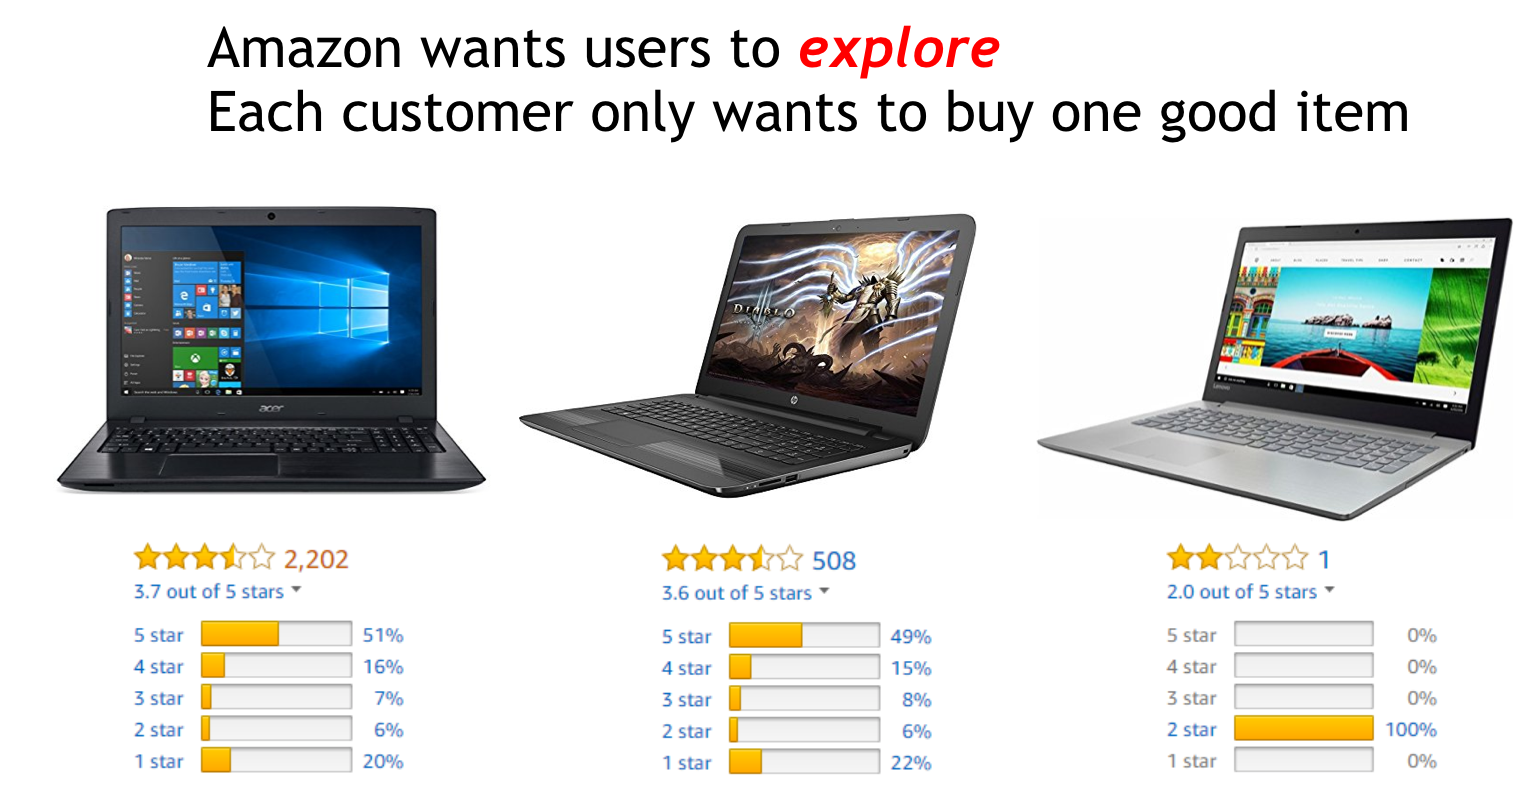
\includegraphics[scale=0.4]{example}
\end{frame}
%#################################################

%#################################################
\begin{frame}{Previous Work}
\textbf{Without Money Transfer}\\
\small{
\begin{itemize}
\item Kremer, Mansour \& Perry 2014
\item Mansour, Slivkins \& Syrgkanis 2015
\item Mansour, Slivkins, Syrgkanis \& Wu 2016
\item Mansour, Slivkins \& Wu 2018
\item Slivkins 2017
\end{itemize}
%Kremer et al. 2014; Mansour et al. 2015, 2016, 2018; Slivkins 2017\\
%\begin{itemize}
%\item %Implementing the “Wisdom of the Crowd”, Kremer et al. 2014;
%\item %Bayesian incentive-compatible bandit exploration, Mansour et al. 2015;
%\end{itemize}
}
\vspace{0.5cm}
\textbf{With Money Transfer}\\
\small{
\begin{itemize}
\item Frazier, Kempe, Kleinberg \& Kleinberg 2014
\item Han, Kempe \& Qiang 2015
\item This paper
% Frazier et al. 2014; Han et al. 2015
%\item Incentivizing exploration, Frazier et al. 2014;
%\item Incentivizing exploration with heterogeneous value of money, Han et al. 2015;
\end{itemize}
}
\end{frame}

%#################################################

\begin{frame}{Heterogeneity presents a new challenge}
\begin{center}
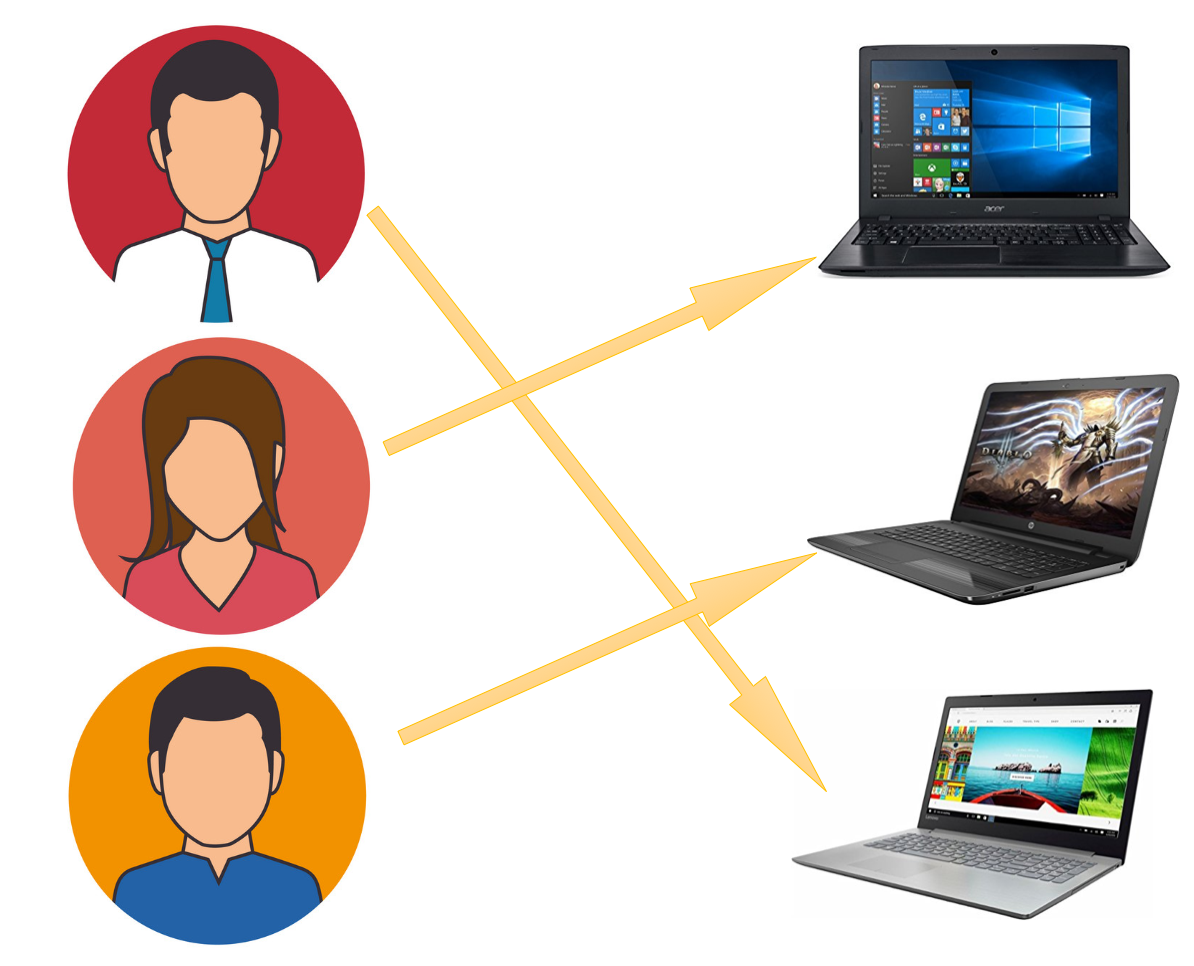
\includegraphics[scale=0.35]{example2}
\end{center}
\begin{itemize}
\item \textbf{Customers prefer different kinds of items}
\item \textbf{Amazon doesn't know which item each user prefers}
\end{itemize}

\end{frame}

%#################################################


%#################################################

\begin{frame}{Heterogeneity Provides Free Exploration}
\begin{itemize} 
\item In the classical MAB: cumulative regret is $O(\log(T))$
\item In incentizing exploration with heterogeneous users:\\ we show, with assumptions, cumulative regret is $O(1)$
\item Key insight: Heterogeneity provides free exploration
\item Our contribution: First algorithm and analysis for incentivizing exploration when users have heterogeneous preferences over arms
\end{itemize}
\end{frame}

%#################################################
\begin{frame}{Problem Setting}

%\textbf{Myopic Agents}
\textbf{Agents}
\begin{itemize}
\item Myopic agents arrive sequentially
\item Agent $t$ has linear preferences with weight vector $\bm{\theta}_t\in \mathbb{R}^{d}$ drawn from known distribution $F$
\end{itemize}
\vspace{0.5cm}

%\textbf{$N$ arms}
\textbf{Arms}
\begin{itemize}
\item Each arm has an unknown feature vector $\bm{u}_i\in \mathbb{R}^{d}$
\item Agent $t$ derives expected value $\bm{\theta}_{t}\cdot \bm{u}_{i}$ from pulling arm $i$
% \item Everyone sees averages $\hat{\bm{u}}_{i,t}$ of noisy 
\item Pulls gives noisy observation of $\bm{u}_i$ 
%{\footnotesize (independent sub-Gaussian noise)}
\item Everyone observes averages $\hat{\bm{u}}_{i,t}$ of each arm's past pulls
\end{itemize}

\vspace{0.5cm}
\textbf{Agents' behavior}
\begin{itemize}
\item Principal chooses payment $c_{t,i}$ for arm $i$ at time $t$
\item Agent $t$ pulls arm $i_t = \arg\max_{i}\{\bm{\theta}_{t}\cdot \hat{\bm{u}}_{i,t}+c_{t,i}\}$
\end{itemize}


%\item Without incentives, agent $t$ would choose the arm maximizing $\bm{\theta}_{t}\cdot \hat{\bm{u}}_{i,t}$.

\vspace{1cm}

\end{frame}
%#################################################

%#################################################
\begin{frame}{The Principal's Goal}

\vspace{1cm}
\begin{itemize}
\item Regret: $r_t = (\max_{i} \bm{\theta}_t \cdot \bm{u}_i) - \bm{\theta}_t \cdot \bm{u}_{i_t}$
\item Payment: $c_t = c_{t,i_t}$
\item \textbf{Principal's Goal}: Incentivize to minimize the cumulative regret while making a small cumulative payment
\end{itemize}

\end{frame}
%#################################################

%#################################################
\begin{frame}{Key Assumptions}
\begin{itemize}
\item (\textbf{Every arm is someone's best}) Each arm is preferred by at least $p$ fraction of users.
\vspace{0.2cm}
\item (\textbf{Compact Support}) $\bm{\theta}$ has compact support.
% contained in $[0,D]^{d}$.
\vspace{0.2cm}
\item (\textbf{Few near-ties}) 
Let $q(z)$ be the proportion of agents with
$\text{Utility(best arm)} \le z + \text{Utility($2^{\mathrm{nd}}$ best arm)}$.\\
Then $q(z)\leq L\cdot z$ for all small enough $z$.
%whose best arm is no better than $z$ + their second best arm\\
%There exists a $\hat{z}>0$, $L$ such that $q(z)\leq L\cdot z$ for all $z\leq \hat{z}$.
% utility difference between their best and second best arm is less than or equal to $z$. 
\end{itemize}

\end{frame}
%#################################################

%#################################################
\begin{frame}{Main Result}
\begin{block}{Theorem 1}

Our policy achieves:
\begin{itemize}
\item expected cumulative regret $O (N e^{2/p} + L N \log^3(T))$,
\item using expected cumulative payments of $O(N^2 e^{2/p})$.
\end{itemize}
\end{block}

Special case: 
When agent preferences are discrete, i.e. $L=0$,
%When $L=0$ (i.e., agents nearly tied between two arms have measure $0$),
regret and payment are bounded by constants in $T$.



\end{frame}
%#################################################

\begin{frame}{Algorithm Sketch}

An arm is \textbf{payment-eligible} if:
\begin{itemize}
\item without incentives, its probability of being pulled is below a threshold
\item AND it hasn't been pulled in a long-time
\end{itemize}
\vspace{0.5cm}

Our \textbf{algorithm}:
\begin{itemize}
\item If there is a payment-eligible arm, offer enough incentive to raise its probability of being pulled above the threshold
\item Otherwise, let agents play myopically
\end{itemize}
\end{frame}

%\begin{frame}{Algorithm}
%
%\begin{algorithmic}
%\STATE Set the current phase number $s = 1$.
%\COMMENT{Each arm is pulled once initially ``for free.''}
%\FOR{time steps $t = 1, 2, 3, \ldots$} {
%\STATE Update the current phase number if needed;
%\IF {there is a payment-eligible arm $i$} 
    %\STATE Offer ''whatever it takes'' payment for pulling arm $i$ (and payment 0 for all other arms).
%\ELSE
    %\STATE Let agent $t$ play myopically, i.e., offer payments 0 for all arms.
%\ENDIF 
%}\ENDFOR
%\end{algorithmic}
%
%\end{frame}


%#################################################
%\begin{frame}{Notations}

%\textbf{Phase}
%\begin{itemize}
%\item Phase $s$ starts when each arm has been pulled at least $s$ times.
%\end{itemize}

%\vspace{0.7cm}
%\textbf{Payment-eligible}
%\begin{itemize}
%\item Arm $i$ has been pulled at most $s$ times up to time $t$;
%\item The conditional probability of pulling arm $i$ is less than $\frac{1}{\log(s)}$ given the current estimates $\hat{u}_{i,t}$.
%\end{itemize}

%\end{frame}

%#################################################
%\begin{frame}{Algorithm}

%\begin{algorithmic}
%\STATE Set the current phase number $s = 1$.
%\COMMENT{Each arm is pulled once initially ``for free.''}
%\FOR{time steps $t = 1, 2, 3, \ldots$} {
%\IF {$m_{t,i} \geq s+1$ for all arms $i$}
%\STATE Increment the phase $s = s + 1$.
%\ENDIF
%\IF {there is a payment-eligible arm $i$} 
%    \STATE Let $i$ be an arbitrary payment-eligible arm.
%    \STATE Offer payment $c_{t,i} = \max_{\theta,i'} \theta \cdot (\hat{\mu}_{t,i'} - \hat{\mu}_{t,i})$ for pulling arm $i$ (and payment 0 for all other arms).
%\ELSE
%    \STATE Let agent $t$ play myopically, i.e., offer payments 0 for all arms.
%\ENDIF 
%}\ENDFOR
%\end{algorithmic}

%\end{frame}
%#################################################


%#################################################
%\begin{frame}{Payment Analysis}
%\textbf{Key technical lemma}: an adaptive concentration inequality (Zhao et al. 2016);
%\vspace{1cm}

%\textbf{Early Phases}: bound by $N$;
%\vspace{1cm}

%\textbf{Later Phases}: exponentially unlikely as the phases advances;
%\end{frame}
%#################################################

%#################################################
%\begin{frame}{Regret Analysis}

%\textbf{When principal incentivizes:} similar to the payment proof;
%\vspace{0.5cm}

%\textbf{When agents pull myopically:} We define a phase-dependent cutoff $\gamma(s(t))$ to further distinguish agents based on the regret.
%\begin{itemize}
%\item $r(t)\geq \gamma(s(t))$:
%\begin{itemize}[label=$\star$]
%\item this happens with exponentially decreasing probability;
%\item since $\theta_t$ has a compact support, the maximum regret is bounded by a constant;
%\end{itemize}
%\item $r(t)\leq \gamma(s(t))$:
%\begin{itemize}[label=$\star$] 
%\item not so many agents have near-ties preferences; 
%\item the maximum regret is bounded above by $\gamma(s(t))$;
%\end{itemize}
%\end{itemize}

%\end{frame}
%#################################################
\begin{frame}{Questions?}
\begin{center}
\Huge{Thanks for your time!}
\end{center}
\end{frame}
%#################################################




\end{document}

